\documentclass[a4paper]{article}
\usepackage{authblk}
\usepackage[]{biblatex}
\usepackage{graphicx}
\usepackage{hyperref}
\usepackage{xspace}
\usepackage{caption,tikzpagenodes,everypage,ifthen}

\newcommand*{\eg}{e.g.\@\xspace}
\newcommand*{\ie}{i.e.\@\xspace}

\addbibresource{bibliography.bib}
\addbibresource{positionpaper.bib}
\title{Establishing RSE departments in German research institutions}

% The file contributors.tex is automatically generated by running contributors.py.
% Changed within will be OVERWRITTEN.
% For changes to the tex template, change contributors.tex.j2.
% For changes to the author information, change contributors.yml.
%
\author[]{Markus Ankenbrand}
\author[]{Bernd Flemisch}
\author[5]{Florian Goth}
\author[3]{Jean-Noël Grad}
\author[2]{Dominic Kempf}
\author[4]{Jan Linxweiler}
\author[]{Axel Loewe}
\author[](Leyla Jael Castro)
\author[](Philipp S. Sommer)
\author[1]{Frank Löffler}
\author[1]{Philipp Matthias Schäfer}
\author[]{Alexander Struck}
\affil[1]{Competence Center Digital Research, Michael Stifel Center Jena, Friedrich Schiller University Jena, Jena, Germany}
\affil[2]{Heidelberg University, Scientific Software Center, Germany}
\affil[3]{Institute for Computational Physics, University of Stuttgart, Germany}
\affil[4]{Technische Universität Braunschweig, Germany}
\affil[5]{Institute for Theoretical Physics and Astrophysics, University of Würzburg, Germany}


\date{\today}

\AddEverypageHook{
  \ifthenelse{\value{page}=2}{\begin{tikzpicture}[remember picture, overlay]\node[anchor=north] at ([xshift=0cm,yshift=0cm]current page marginpar area.north){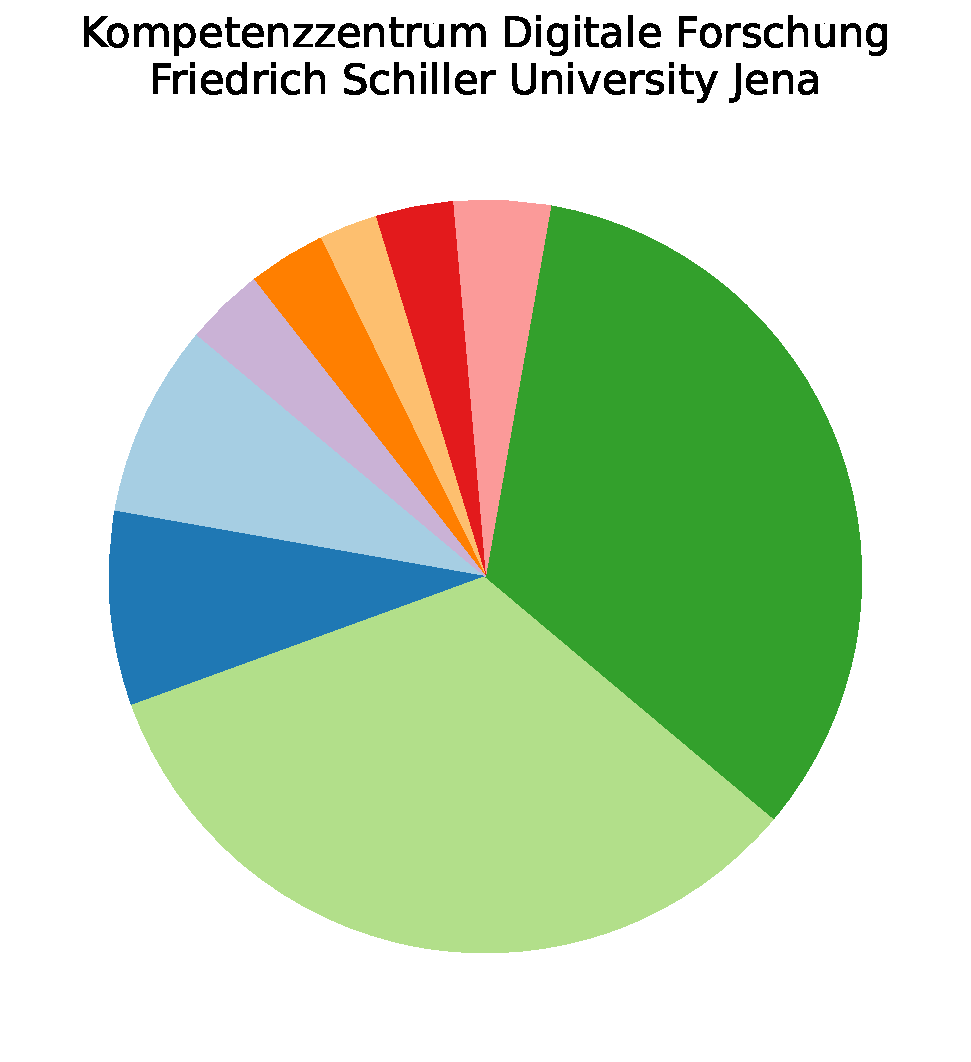
\includegraphics[width=\marginparwidth]{group_composition_plot/pdf/Friedrich_Schiller_University_Jena_2023-12-06_10-43-44}};\end{tikzpicture}}{}
  \ifthenelse{\value{page}=3}{\begin{tikzpicture}[remember picture, overlay]\node[anchor=north] at ([xshift=0cm,yshift=0cm]current page marginpar area.north){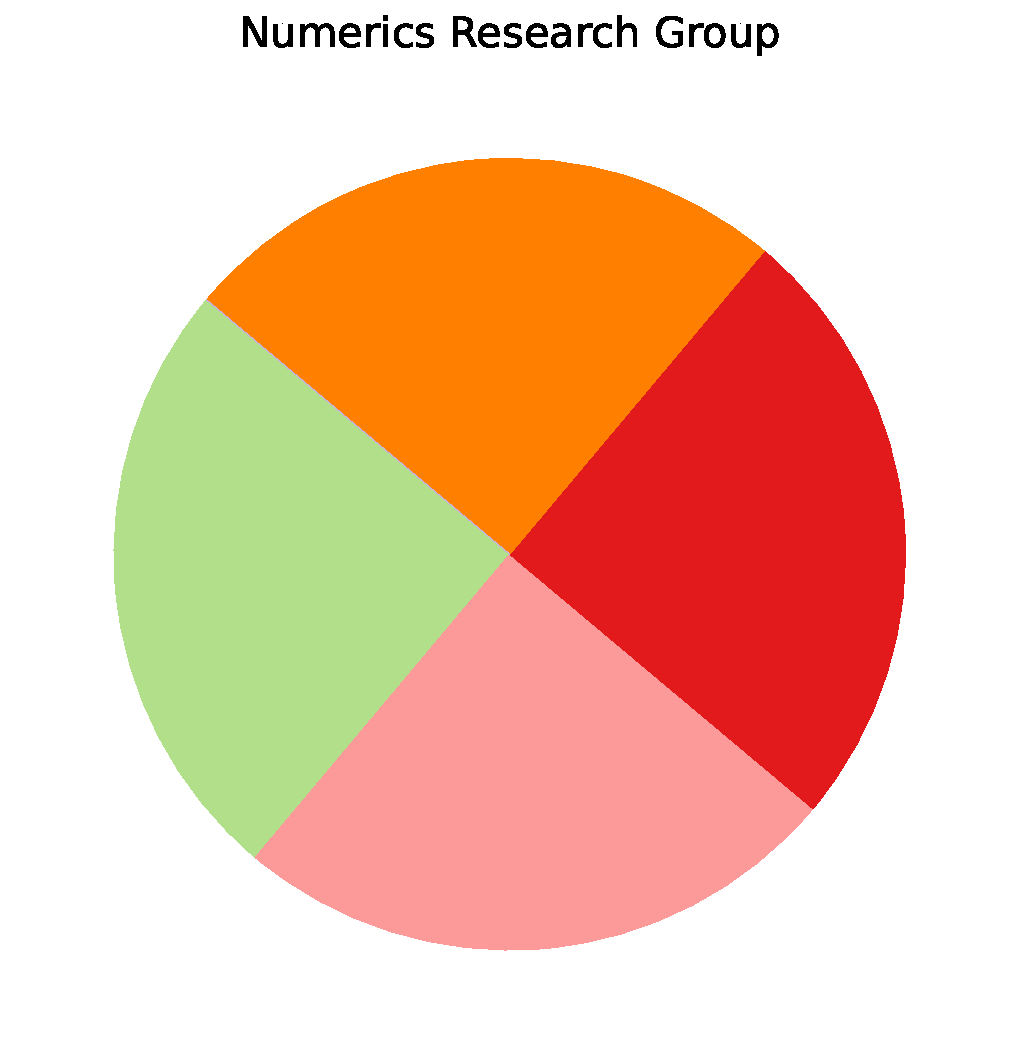
\includegraphics[width=\marginparwidth]{group_composition_plot/pdf/Numerics_Research_Group_2023-11-30_08-35-53}};\end{tikzpicture}}{}
  \ifthenelse{\value{page}=4}{\begin{tikzpicture}[remember picture, overlay]\node[anchor=north] at ([xshift=0cm,yshift=0cm]current page marginpar area.north){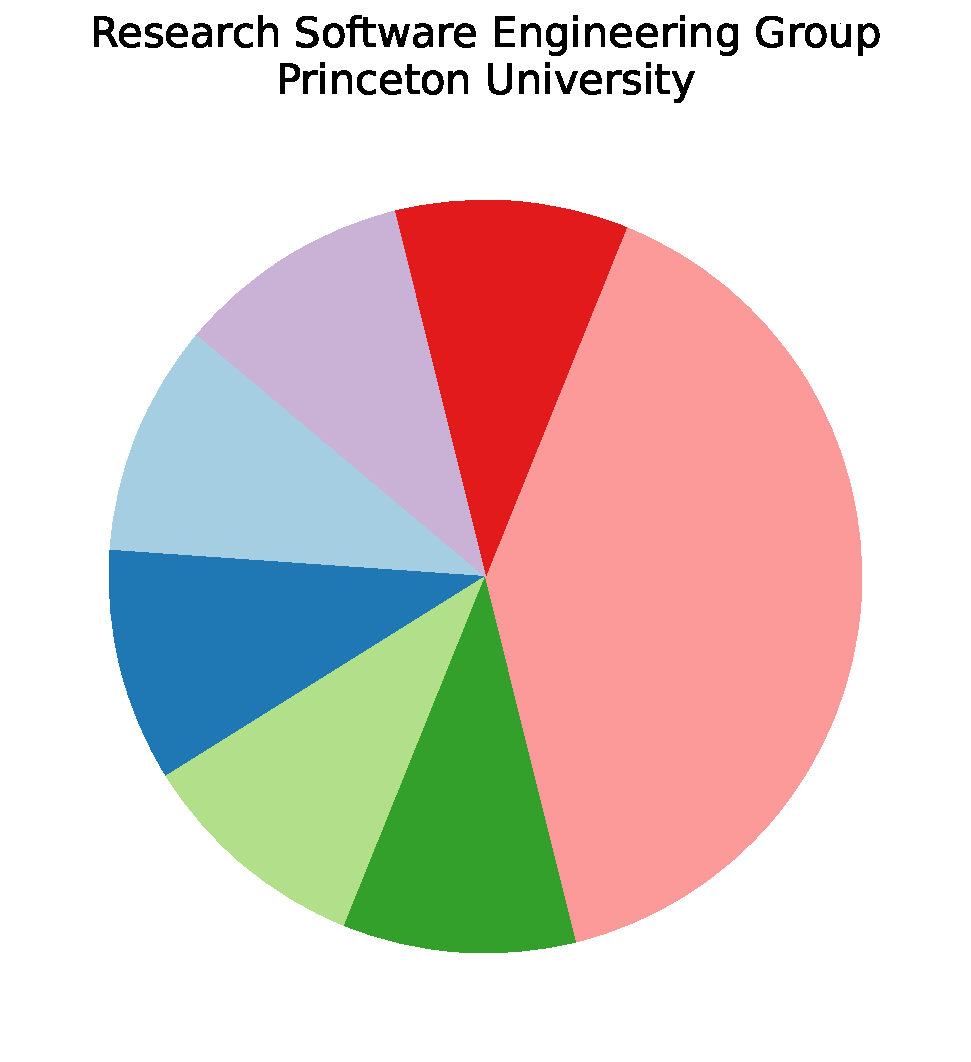
\includegraphics[width=\marginparwidth]{group_composition_plot/pdf/Princeton_University_2023-11-29_18-33-21}};\end{tikzpicture}}{}
  \ifthenelse{\value{page}=5}{\begin{tikzpicture}[remember picture, overlay]\node[anchor=north] at ([xshift=0cm,yshift=0cm]current page marginpar area.north){\includegraphics[width=\marginparwidth]{group_composition_plot/pdf/Project_Z03_uni_würzburg_2023-11-24_11-21-07}};\end{tikzpicture}}{}
  \ifthenelse{\value{page}=6}{\begin{tikzpicture}[remember picture, overlay]\node[anchor=north] at ([xshift=0cm,yshift=0cm]current page marginpar area.north){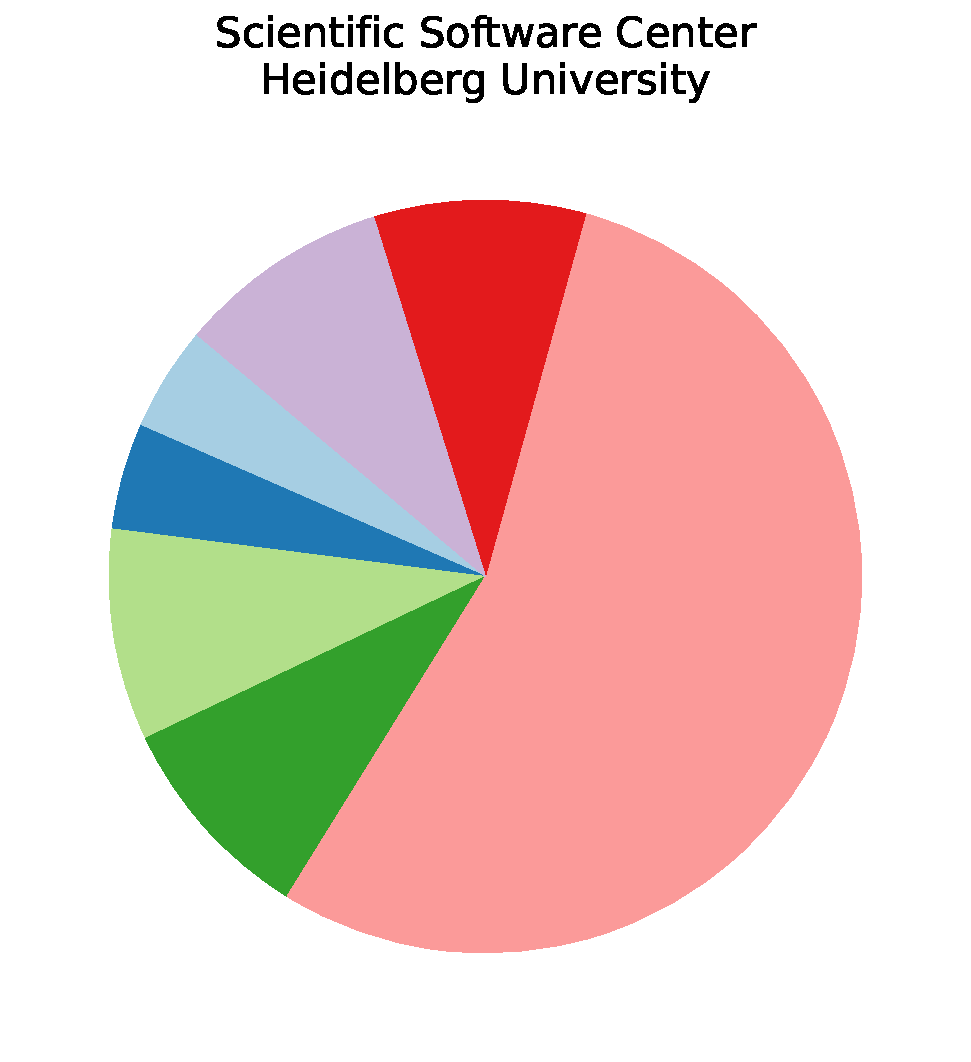
\includegraphics[width=\marginparwidth]{group_composition_plot/pdf/Scientific_Software_Center_2023-12-21_13-13-27}};\end{tikzpicture}}{}
  \ifthenelse{\value{page}=7}{\begin{tikzpicture}[remember picture, overlay]\node[anchor=north] at ([xshift=0cm,yshift=0cm]current page marginpar area.north){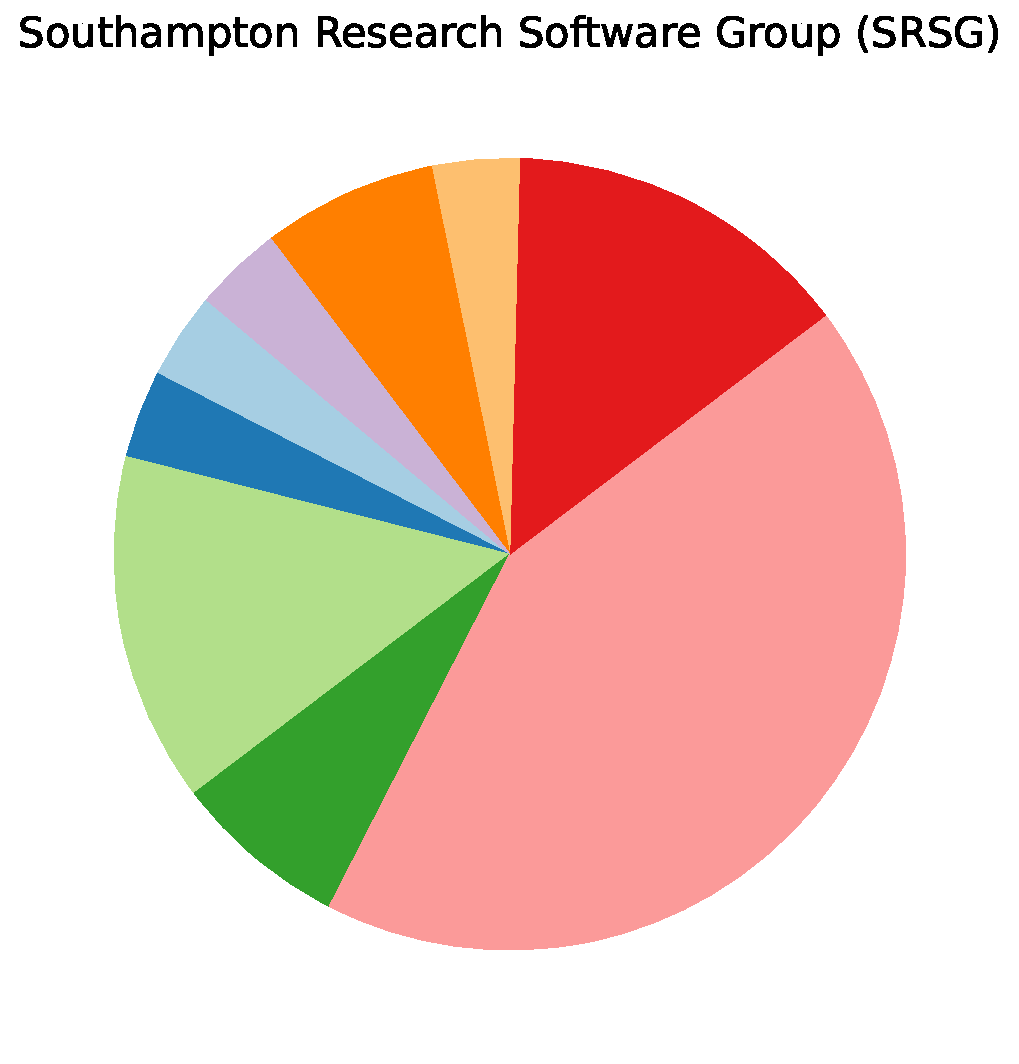
\includegraphics[width=\marginparwidth]{group_composition_plot/pdf/Southampton_Research_Software_Group_SRSG_2023-11-25_14-33-57}};\end{tikzpicture}}{}
  \ifthenelse{\value{page}=8}{\begin{tikzpicture}[remember picture, overlay]\node[anchor=north] at ([xshift=0cm,yshift=0cm]current page marginpar area.north){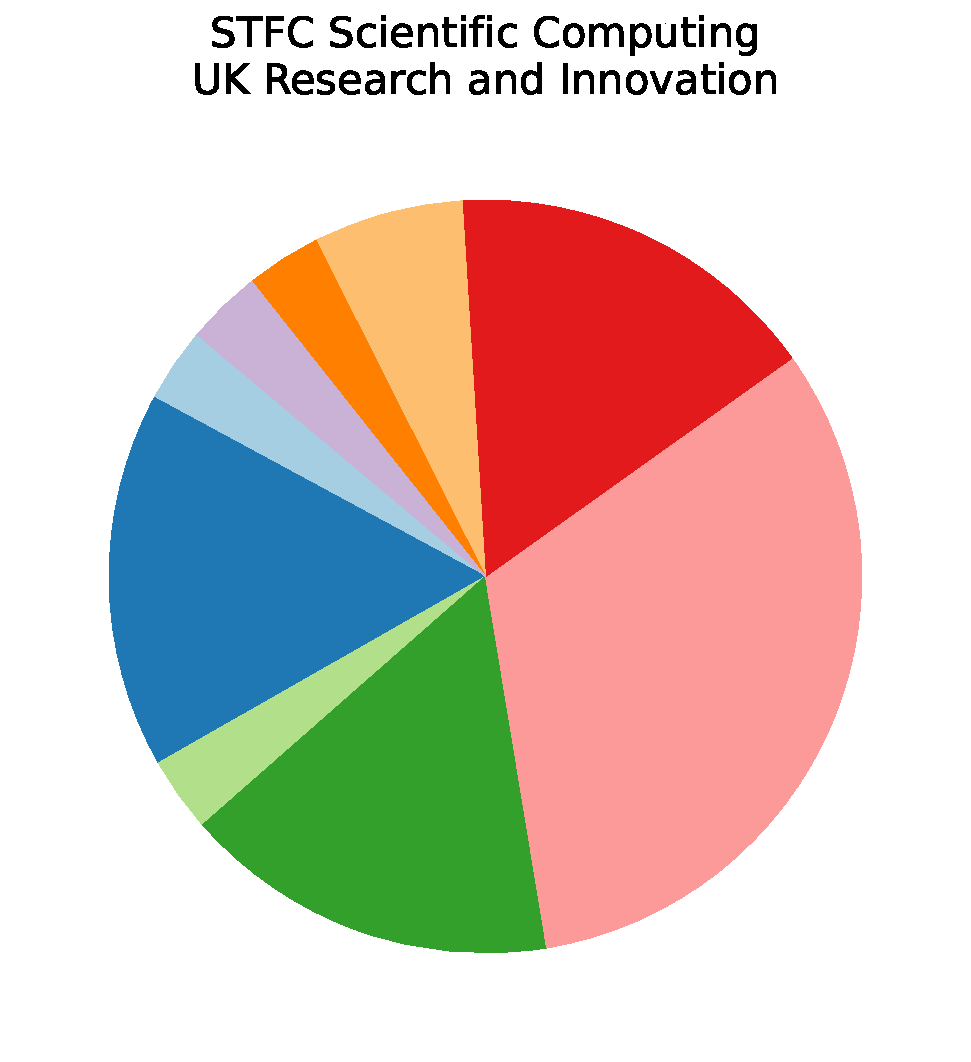
\includegraphics[width=\marginparwidth]{group_composition_plot/pdf/STFC_Scientific_Computing_part_of_the_UKRI_2023-11-24_12-05-38}};\end{tikzpicture}}{}
  \ifthenelse{\value{page}=9}{\begin{tikzpicture}[remember picture, overlay]\node[anchor=north] at ([xshift=0cm,yshift=0cm]current page marginpar area.north){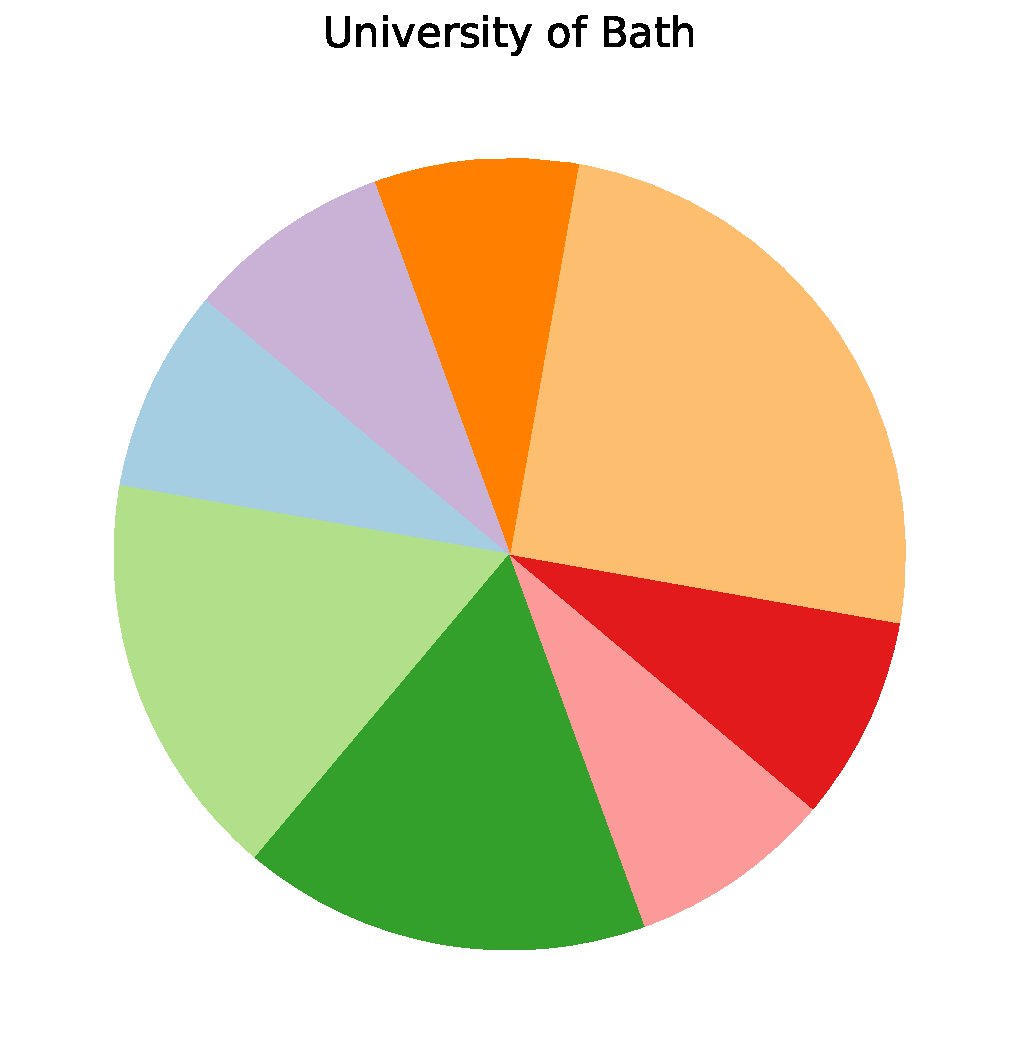
\includegraphics[width=\marginparwidth]{group_composition_plot/pdf/University_of_Bath_2023-12-08_16-21-44}};\end{tikzpicture}}{}
  \ifthenelse{\value{page}=10}{\begin{tikzpicture}[remember picture, overlay]\node[anchor=north] at ([xshift=0cm,yshift=0cm]current page marginpar area.north){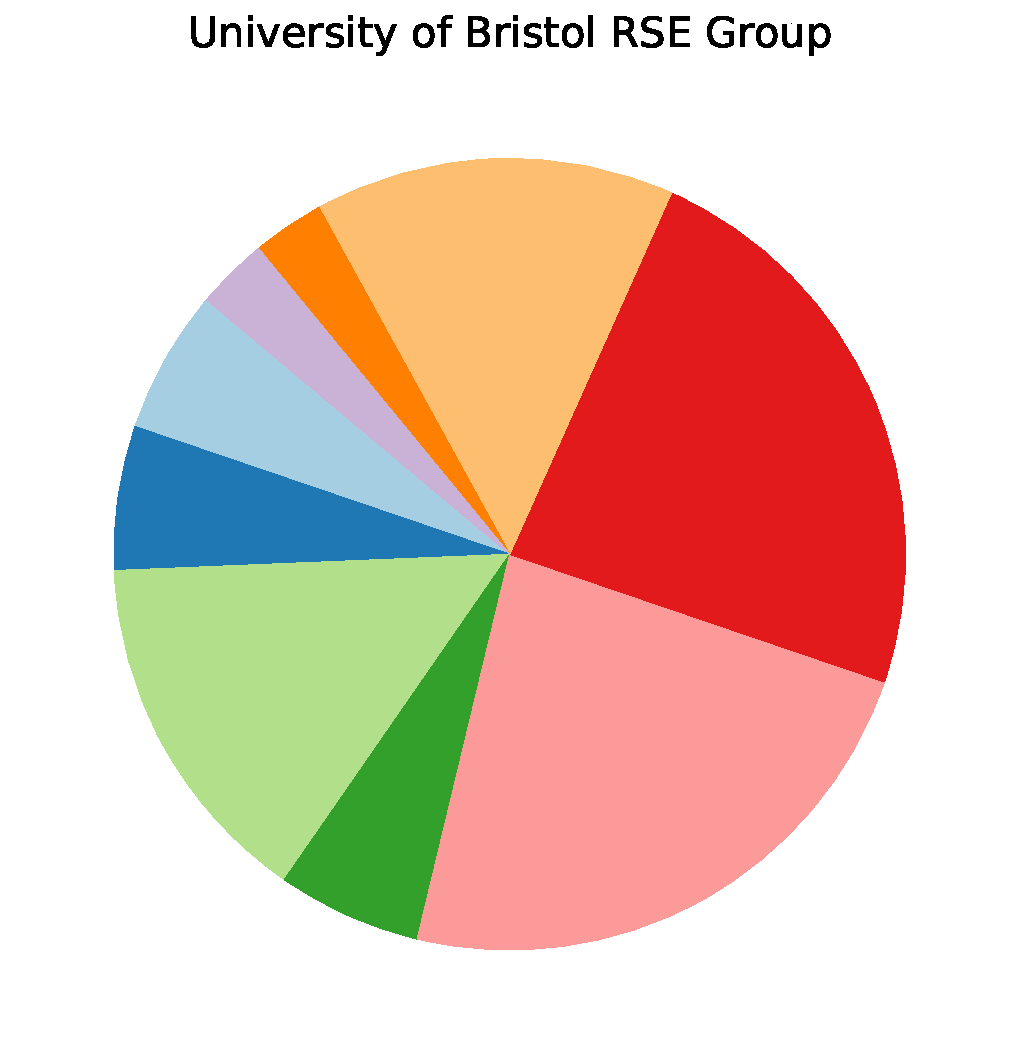
\includegraphics[width=\marginparwidth]{group_composition_plot/pdf/University_of_Bristol_RSE_Group_2023-11-27_10-13-46}};\end{tikzpicture}}{}
  \ifthenelse{\value{page}=11}{\begin{tikzpicture}[remember picture, overlay]\node[anchor=north] at ([xshift=0cm,yshift=0cm]current page marginpar area.north){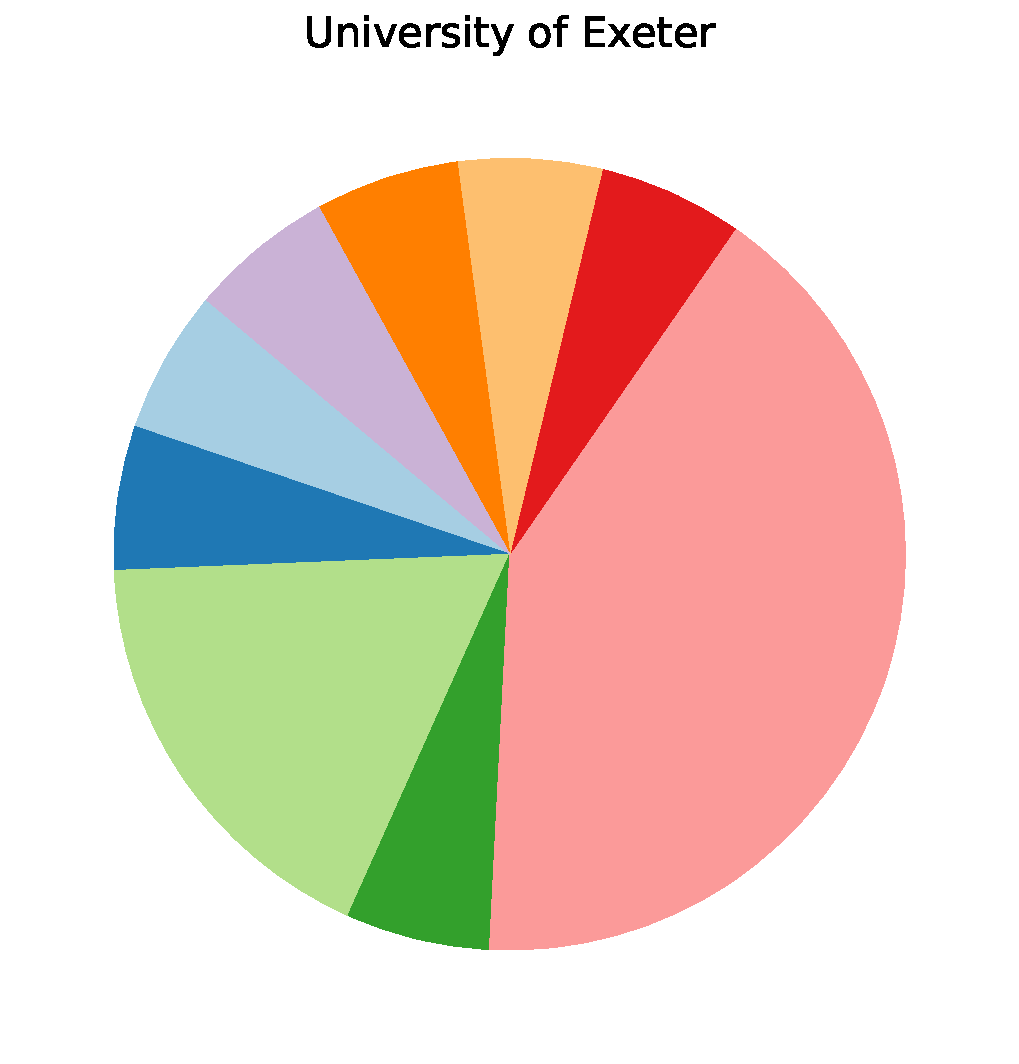
\includegraphics[width=\marginparwidth]{group_composition_plot/pdf/University_of_Exeter_2023-11-24_11-49-44}};\end{tikzpicture}}{}
  \ifthenelse{\value{page}=12}{\begin{tikzpicture}[remember picture, overlay]\node[anchor=north] at ([xshift=0cm,yshift=0cm]current page marginpar area.north){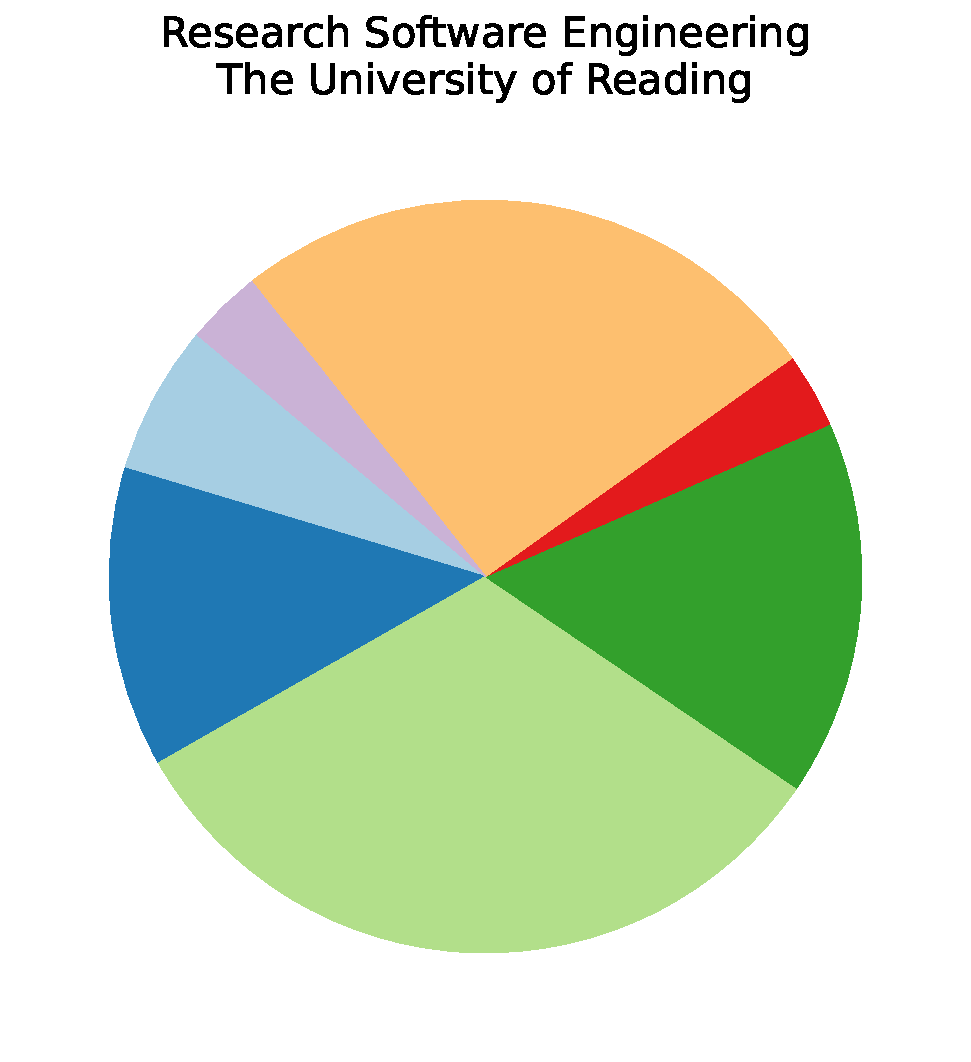
\includegraphics[width=\marginparwidth]{group_composition_plot/pdf/University_of_Reading_2023-12-11_10-18-14}};\end{tikzpicture}}{}
}



\begin{document}

\maketitle

\section{Introduction}
Research software has been written and used for decades in a range of disciplines.
It has been established that most research requires research software for its results~\autocite{Hannay2009, Hettrick2015}.
To solve pressing research challenges, better software is crucial~\autocite{Goble2014}.
During the past decade, it gained ever-growing attention and is becoming accepted as a research result on its own.
%We follow here the definition: “Research Software includes source code files, algorithms, scripts, computational workflows and executables that were created during the research process or for a research purpose”, with full definition and discussion provided in~\autocite{Gruenpeter2021}.

The number of people developing software in academia is constantly rising~\autocite{Hannay2009, Hettrick2015}.
Research Software Engineering consists of actions necessary to create, adapt or maintain Research Software or train others to do so.
These actions are very diverse and so are the environments they are performed in.
This position paper focuses on (groups of) research software engineers and researchers who require RSE for their research.
We advocate the establishment and support of dedicated, central RSE groups in German research organizations, with clearly defined tasks, contact points, and, in particular, sustained funding.
We provide an overview of the various task these teams have and discuss potential realization strategies, learning from already existing examples of such an RSE unit.

Before we motivate the topic of this position paper further, we first introduce the terminology used throught this work.
Depending on the national research
environments and processes that readers are familiar with, the notion of the terms \emph{software} and \emph{research} might differ.
The term “Research software” is also defined somewhat differently within the community.
Therefore, to avoid ambiguities, we define them as follows:\\
\textbf{Software:}\\
Source code, documentation, tests, executables
and all other artefacts that are created by humans during the development process
that are necessary to understand its purpose.\\
\textbf{Research software:}\\
Foundational algorithms, the software itself,
as well as scripts and computational workflows that were created
during the research process or for a research purpose, across all domains of research.
This definition is broader than in~\autocite{FAIR4RS} and is the outcome of a recent
discussion in~\autocite{Gruenpeter2021}.\\
\textbf{Research software engineers:}\\
People who
create or improve research software and/or the structures that the software interacts with
in the computational ecosystem of a research domain.
They are highly skilled team members who may also choose to conduct their own research as
part of their role.
However, we also recognise that many RSEs have chosen specifically to focus on a technical
role as an alternative to a traditional research role because they enjoy and wish to focus
on the development of research software.\\
\textbf{Researchers:}\\
We refer by researchers to all others involved in research or in research supporting organizations such as \eg libraries,
hence those that are at most sporadically performing RSE actions.

Furthermore, we will use the general term \textbf{RSE Hub} for the central RSE team throughout this paper. 
These RSE Hubs can take the form of, e.g., full RSE departments, smaller RSE groups, Open Source Program Office (OSPOs), virtually across multiple units or combined under one single leader, depending on the evironment of the particular research organization under consideration.
All of these implementations are considered here, taking into account the large variety of research environments in Germany.

\section{Motivation}


\begin{quotation}
      \textit{Better Software, Better Research}\\(Mission statement of the UK Software Sustainability Institute)
\end{quotation}

In this chapter, we motivate dedicated RSE groups in German research organizations.
Several stakeholder perspectives are discussed and supported by (inter)national examples, including that of RSEs within RSE groups, RSEs embedded in research groups, Researchers in need of RSE resources, organizational management and that of funders.

We will draw parallels to research data here, because both, data and software, play a fundamental role in all of the research. Over the past decades, Research Data Management (RDM) has evolved into a topic of national interest with NFDI consortia for all disciplines and a research data law. 
Federal state RDM initiatives\footnote{\url{https://forschungsdaten.info/fdm-im-deutschsprachigen-raum/deutschland/}} accelerate the topic further and provide regional training, networking and other supporting services. 
Many research organisations have established central RDM groups that support research projects in all aspects from grant proposals to hands-on support and maintaining Data Management Plans (DMP). 
Funding agencies acknowledge the importance of research data and started to make RDM mandatory in research projects. 
Due to the similar nature of both, data and software, and their importance in today's digital research, it is reasonable to expect a similar trajectory in the development of research software as a topic.
%such output has become more important over the last two decades. Since research software can be considered valuable research output as well, we expect a similar trajectory for software.
%gh training researchers, the reusability through data repositories and to avoid duplication of effort.
%For over a decade, research funders and organizations made a significant effort to establish RDM and teams around it, for example the Utrecht University Research Data Management Support~\autocite{UtrechtRDM}, University of Stuttgart FoKUS team~\autocite{Boehlke2024} or TUBS.researchdata~\autocite{Grunwald2022} at TU Braunschweig.
%We assume that research software will follow a similar trajectory.
%\footnote{For arguments when research software is unlike data, see \autocite{Lamprecht2020}.}


While we focus on Germany here, it is beneficial to review how other countries approach research software.
In the UK, for example, many universities started initiating dedicated RSE departments about a decade ago~\autocite{Crouch2013}.

\subsection{Tasks}

One of the services a centralized RSE department likely will provide is training to improve the often low-quality code developed by beginners [REF low-quality].
Examples of organizational training efforts are the Helmholtz HIFIS group [https://events.hifis.net/category/4/], the Scientific Software Center in Heidelberg [https://www.ssc.uni-heidelberg.de/en], the Competence Center Digital Research in Jena (zedif: [https://www.zedif.uni-jena.de/en/]), and the SURESOFT workshops series in Braunschweig ~\autocite{SURESOFTLink, Blech2022}.
Another national pioneer is the Göttingen State and University Library which set up a group of RSEs offering – besides training – services like data modeling and visualization, digital editions, portal development and more. They reported a remarkable increase in software quality, better grant applications, less brain drain and overall employee satisfaction levels~\autocite{schimavoigt2023}.
The demand for such services appears to be ever-increasing.
Other tasks include code review (REF? Charite), consultation services regarding frameworks or algorithm selection, licensing, and more. 
RSEs have always embraced and supported collaborative infrastructure and tools, e.g. GitLab, Containerisation, etc. and thus enabled fellow researchers utilising such infrastructure. 
In some national and international organisations, established RSE groups already develop solutions for (and guided by) research projects. This approach assures high quality research software and allows domain scientists to focus on their research challenges. 
This is likely to save time and accelerate publication of results.



\subsection{Structure}

A central RSE team on long-term contracts will act as a knowledge hub due to their experience in and support of several disciplines as well as established contacts within the organisation.
This is comparable to commercial/industry R\&D departments, where key software architects and developers establish a knowledge hub and consult with as many projects as necessary [REF].
Subject matter experts like software architects, database administrators and other tooling specialists are organized centrally and share their knowledge by consulting with decentralized projects. It makes economically sense to organise such personel as cost-effective as possible since not every project can afford or needs such RSE FTEs. 
Most academic research organizations have established centralized tooling, e.g. storage or HPC, but only a few consider software development and consultancy a relevant service yet. 
RSE departments act as knowledge hubs in a network of academic developers within an organisation~\autocite{Elsholz2006}.
This enables the embedded experts to maintain in-depth knowledge and to assess current trends and developments, both in research as well as technology.

RSEs in centralised groups are interdisciplinary specialists due to their experience working on diverse topics, as well as overlaps in methodology across disciplines and research software in general.
They are assumed to be able to suggest the most appropriate tools/frameworks and design or architecture patterns for certain research challenges.
Their diversity in skills (languages, frameworks, front/back-end, UX, management) is welcomed, especially for short-term needs in projects.
This will save money often spent in a duplication of effort.
Furthermore, given appropriate long-term funding, a central RSE hub will be able to keep essential software alive, even if it was developed in short-term projects.
%Such code often requires long-term maintenance, support, new features or bug fixes.
%The decision of curation is commonly based on measures that involve quality, academic or societal impact among many others.


Coming back to RDM again for comparison: The most recent funding guidelines suggest “data stewards” in data-driven research.
Such experts are to be employed in advanced research projects like “Collaborative Research Centers” (CRC) \footnote{Sonderforschungsbereich (SFB)} or “Clusters of Excellence”
\footnote{Cluster der Exzellenzinitiative}.
These data experts support research projects in several aspects including DMPlans, grant applications, data availability for journal publications, compliance, FAIRification and more.
Similarly, RSEs will encourage scientists to publish software with rich metadata and will support journal publications with code submission requirements.
With the increasing recognition of software as a research object/result, it is easy to see how projects will require and benefit from support in software needs in the near future.


The Carpentries~\autocite{Carpentries} exemplify a similar success story [REF SuccessStory Carpentries https://carpentries.org/testimonials/]. Requests or suggestions for even more training show the need for such services.
RSE services which benefit all disciplines/departments may represent a unique selling point for organizations competing for the brightest minds.
See the examples from leading universities above.

Given that RDM training or coordination is a centralized effort in most organizations, the time has come to implement a similar structure for research software services.
Such a group may extend or include RDM or collaborate with such service teams.
See the Vision and Realization sections below for more details.

\subsection{International Comparison and Current Developments}


Selected research institutions in the UK have pioneered the deployment of RSEs into research projects~\autocite{Crouch2013}. The successful establishment of such staff is a role model for similar academic organizations worldwide.
A range of already-existing departments can be seen in this map: https://society-rse.org/community/rse-groups/

In the UK, for example, almost all grant applications include software development in their budget.
This allocated money can then be utilized to delegate/dispatch a central RSE person or group into a research project for a few weeks or months as necessary.

We welcome that the latest DFG grant application templates require discussion of both, data \textbf{and} software management (in line with their GWP guidelines~\autocite{dfg_gsp}).
%We also see the first grant applications [REF welcome trust? or others] requiring Software Management Plans (SMP).
In addition, dedicated Data Management Plans (DMP) have become mandatory in several funding calls (e.g., ...) and we expect to see a similar development for SMPs in the future. (There have been funding calls in the UK that required a SMP. [no ref?]) 

Policies for research software management and guidelines involving responsible research practices detailing software handling are the precursors for a research software engineering environment.
See for example position papers by the Helmholtz Open Science Office~\autocite{Helmholtz2019a,Helmholtz2019b},
the AllianzInitiative~\autocite{Konrad2021},
the University Utrecht~\autocite{Utrecht2016b},
and the German Research Council~\autocite{dfg_gsp}.
%% TODO: Double-check that DLR guidelines are referenced.

Another development taking place worldwide is the encouragement of authors to submit both, data and software, for peer review. As an example, the journal "Nature" initiated such a policy\footnote{\url{https://www.nature.com/nature-portfolio/editorial-policies/reporting-standards}} in 2018~\autocite{Nature2018}.
RSE groups are able to offer researchers consulting tailored to their specific needs on how to implement and document those policies.

The global FAIR movement originated from RDM and widened their focus to include research software.
However, it also has become clear in that process that software is not “just another type of data" and, e.g., the FAIR principles are not sufficient for software.
The FAIR principles for Research Software (FAIR4RS)~\autocite{ChueHong2022} have been adopted worldwide~\autocite{Barker2024}, including the German Ministry of Education and Research (BMBF) and the German Research Foundation (DFG).
% adoption of FAIR4RS (inter)nationally
The rather complex assessment of FAIRness~\autocite{Wilkinson2023,FAIRmaturity} has also widened from data to software~\autocite{Lamprecht2020}.

%\subsection{Better Software, Better Research}
%Such software is assumed to have a much longer life cycle and may be more evolvable or extensible due to better code quality and architectural decisions that ease reuse.

\subsection{Towards a Thriving Future}

In conclusion, we observed that RSE groups already do support research software development, publication, and development among many important tasks. 

%Publication efforts for better software will increase discoverability which in turn will decrease duplication of effort.
%Scarce resources like professional staff, time and money are not put to waste. 
%Instead, better software (publications) will lead to outstanding reputation.

A professionalization in software development and management can be expected to improve the transition from prototypes to software products.% to the benefit of everyone.
Less technical debt \footnote{\url{https://www.gartner.com/en/information-technology/glossary/technical-debt}} will be amassed, which is beneficial for reuse.

High-quality software is likely to be published, cited, and reused.
Better software is assumed to have a much longer life cycle and may be more evolvable or extensible due to better code quality and architectural decisions that ease reuse.
This will benefit researchers, organizations, funders, and society.

%Necessary software management activities like (git-based) version control are assumed to improve collaboration among researchers.




% move to vision
%Software development and management training efforts included in the "studium generale" (or similar education strategies) will further the knowledge of students and early career researchers.

%In contrast, organizations lacking such RSE knowledge need to purchase professional support - in the industry often realized via consulting.
%Academic research hardly has the resources to compete for effective consulting.
%Academic research is assumed to aim for sovereignty and independence of third-party providers.

\section{Vision}
\label{sec:vision}
In the following, we describe our vision of central RSE departments at research institutions in Germany.
As these institutions include universities, other colleges, as well as large associations like Max-Planck, Helmholtz, Fraunhofer or Leibniz,
they show a wide variety in organizational structure as well as internal scientific diversity.
Thus, there can be no single optimal concept of such a department for all research institutions in Germany.
We instead describe modular components that can be mixed and matched based on the respective local environment.

These suggested nine modules comprise the core services of an RSE department.
Not all, and probably not even most of the RSE departments will deliver all nine, and different RSE departments will focus on different modules.
Thus, it is likely that no two departments will be, or should be, alike.
However, these nine modules together with assumed weights are part of a simple model of an RSE group which provides both a quick overview of an individual group as well as a way to compare groups.
The nine modules are decribed in the following.

\subsection{Module 1: Foster a Network of RSEs}
\label{sec:network}

One of the core responsibilities of an RSE department is to act as a coordinator of RSE activities within the institution.
At virtually every academic institution there are employees that assume at least part-time the role of an RSE, with tasks within only a part of that organization.
These decentralized RSEs typically work isolated from similar RSEs in different groups, within the same institution.
A central RSE department provides a condensation core and connects decentralized RSEs with each other and with the ones at the hub.

Connecting decentralized RSEs has multiple, positive effects.
It will enable them to get to know others in similar situations and to learn from as well as support each other.
Contact with the central department will also help RSEs to professionalize their software development, which will directly benefit not only themselves but also their research groups.
In addition, the networking opportunities allow the distribution of knowledge about tools and resources within network partners, including the central RSE department.
There are many RSE skills mastering which can take many years; time that a part-time RSE usually can not spare.
A central RSE department can make sure to connect decentralized RSEs to others with the relevant expertise or offer it themselves.
Fostering the network also enables the department to monitor institutional RSE activities, thereby giving it the insight necessary to prevent duplication of work and support synergies.

How an RSE department realizes this task will depend heavily on its environment and resources. We only mention a few examples here to provide inspiration, with the explicit claim of incompleteness.
These include talks, seminars, workshops, meet-ups, hackathons, as well as informal regulars' tables.
As a foundation, a central RSE department employs experienced RSEs, mostly at the post-doctoral level, who are not only expert software engineers, but also good communicators with the ability to work interdisciplinarily.
At least a core of a central RSE department's employees need to have permanent contracts to be able to offer that deep expertise that requires years of experience.
Moreover, an onboarding process can serve as an entry point for new RSEs, whether decentralized or in the central RSE department, into an institution's network.
This gives an opportunity to gauge how the new colleague can benefit from the department's teaching services and whom they might want to network with based on their planned work.
Similarly an off-boarding process can help to make sure that all acquired knowledge that is relevant to the institution is passed on to someone who stays, even when within a single research group alone that might pose a problem.

\subsection{Module 2: Consultation Services}
\label{sec:consultation}

With the majority of researchers being self-taught programmers [REF], there is a huge demand for expertise on how to develop better research software.
Here, "better" can refer to a number of quality metrics such as correctness, reproducibility, maintainability, extendability, usability, portability, interoperability, performance or scalability [REF].
In order to raise the quality standards for research that is based on research software, it is of great importance for research institutions to provide access to such expertise with a low entry barrier.
The hub is a natural place to provide this central service.
There exists a number of scenarios where RSE consultation services differ strongly in scale and format.
We mention a few of these in the following.

"One Off" consultations on any research software related aspect that are open to researchers of all career levels are
a great introduction to the hub's RSE services and are offered by almost all RSE departments already established [REF].
Depending on the demand, these consultations can either be by appointment or in a more structured format where you book an appointment from available dates (e.g. University of Sheffield's "Code Clinic" [REF]) .

A larger scale format for RSE consultation services could be that a research project regularly (e.g. quarterly or monthly) meets with an RSE in order to coordinate the research software efforts done in the research project.
This format enables valuable feedback cycles between researchers and RSEs and allows RSEs to guide the project
towards successful software engineering best practices without overloading the researchers with information at a one-off consultation.
When an RSE department carries out many of these project consultations, they will gather valuable experiences in transferring RSE knowledge to practitioners.
Having an RSE hub puts these experiences into institutional memory, allowing for better RSE practice in the future.

RSE consultation services are also of great importance in proposal writing.
Many proposals critically depend on research software to be developed and the requirements of funding agencies w.r.t. research software are growing and will continue to do so.
Similar to dedicated RDM units that provide institutional support for data management plans,
the RSE hub can support researchers by providing expertise with software management plans and the software engineering best practices required by these plans.
With consultation services already involved in the proposal phase, improved proposal acceptance rates can be expected [REF], thereby amortizing the investment into RSE departments.


\subsection{Module 3: Development Services}
\label{sec:development}

There is a huge demand for the development and customization of research software tailored to the needs of specific research projects.
Often, the correct solution to this is to educate researchers to write their own software according to RSE best practices.
However, there are also many instances where the knowledge gap between the researchers and the intended research software development is too large to bridge efficiently.
In these cases, RSE development services are a great opportunity that can have a huge impact on the digitization of science at a research institution.
Similar to consultation services, this service can be offered at multiple scales.

Many times, even a small effort of a skilled RSE can have a huge impact on a research project that requires dedicated research software development.
With the leverage of these projects being usually very high, realizing as many of them as possible gives a great boost to the research institution.
Many existing RSE departments (\eg Manchester, Heidelberg) offer this type of small scale service free of charge and use it to promote their services within the institution.

For research projects requiring more substantial software development resources, an RSE department could - either through the hub or its spokes - provide the required developer capacity.
This is especially relevant if the researchers hired for the research projects do not have the required software development skills and the volume of the development is too small to hire a dedicated developer.
Depending on the scale of the involvement, the RSE department can either be included into the grant proposal via a co-PI or as an internal service provider.

If the research within the institution heavily relies on specific pieces of software,
sustaining these pieces is of vital importance for the long term success of the institution.
Relying on a workforce that is subject to academic labor turnover poses a risk of knowledge loss.
If the development is done in an RSE department, institutional memory about critical research software infrastructures can be created and the long term availability of these infrastructures can be improved.
This applies both to domain-specific research software (e.g. simulation frameworks widely used throughout the institution)
and to domain-agnostic software and data infrastructure (\eg Jupyter, workflow management systems, data repository software).

While all of the above development services can be flexibly performed either at the RSE hub or its spokes, there are advantages of having a hub in the process:
It allows building up highly specialized technical expertise with a long term perspective and reuse it across the entire institution.
Examples of topics that would benefit from such expertise pooling are \eg mobile app development and UI/UX development.

RSE departments that offer development services at all scales have proven to be a success story at many research institutions and have rapidly grown in size due to the influx of third party funding.
Notable examples are \eg Manchester [REF], Notre-Dame [REF], STANFORD, Princeton~\autocite{Cosden2022a}.

[SuccessStory]
Founded in January 2017, the Research Computing department of Princeton University has experienced a tremendous growth from the initial two FTEs to a total of 18 FTEs in the span of five years~\autocite{Cosden2022a}.
This growth is based on a continuous influx of new funded projects once successful projects showcase the additional value of RSE services to researchers.

[Success Story]
The University of Manchester Software and Data Science group has successfully established specialized development services within their institution:
The "Mobile Development Service" \autocite{manchester_mobile} team consists of RSEs that focus solely on developing and deploying mobile apps.
Without a central RSE department to anchor such specialized expertise, it would probably be infeasible to establish such a service.
Also, having this expertise centralized allows for synergies in the deployment procedure for mobile apps:
The RSE department can create institutional accounts with the app stores and manage the time consuming deployment process including hard-to-setup procedures like code signing.
Besides the technical benefits of this central deployment procedure, the institution will also benefit from the increased visibility and potentially be able to build a brand with its technological output.

\subsection{Module 4: Teaching Services}
\label{sec:teaching}

A central RSE department can provide or organize training for researchers and decentralized RSEs in an institution.
This can replace self-education for foundational software development skills and provide a basis from which researchers can continue to learn more specialized skills guided by experts of the central department.
It also improves the quality of much of the fairly simple software being written by researchers; scripts to process and maybe visualize their data.
As teaching material for foundational software development skills is freely available,
the tasks remaining for a central RSE department are to adapt the material to local requirements as well as to organize and hold courses and workshops.

For more complex software development projects, a central RSE department can offer individual teaching, either through consultation or by lending out RSEs into projects of research departments.
In both cases the expert RSEs from the central RSE department can pass on their knowledge precisely adapted to the concrete needs of those that they support.

\subsection{Module 5: Create a Network of Institutional Partners}
\label{sec:partners}

Within a research institution, a lot of groups or departments touch the topic of research software one way or another.
However, their coverage of RSE-related needs of researchers is often limited and their main responsibility typically lies elsewhere.
While this is one of the main arguments for the creation of dedicated RSE departments, it also shows the necessity for an RSE department to closely interact with its respective partners.

In the following, we describe groups or departments that can typically be found within academic organizations,
what usually their focus is and how we envision collaborations with an RSE department.
However, note that as research organizations can differ widely from one another, so can the tasks and even existence of the entities below.
Arguments and conclusions below have to be adapted to specific circumstances when applying them to specific environments.

All research institutions in Germany do have a computing center of one form or another.
At the very least, these are the persons that deal with the every-day IT-need of the institution:
Internet access, Email, Web, central administration of computers (at least that of administrative staff), etc.
Typically, the assigned tasks of the computing center are not research-driven, or also the staff does not have a research background.
However, research software often has to work within the environment provided by the computing center.
A central RSE department can help to either adapt the research software or even the environment such that the needs of researchers can be met.
It is not unusual that this requires a level of engagement and understanding of the underlying research concepts that the staff of the computing center cannot provide alone.

A second important partner is the local library, which has already gained tasks much beyond the preservation and organisation of publications on physical paper for quite some time.
Besides digital forms of rather traditional publications, these more and more include digital data and recently also software publications, their discovery and citation.
With the dedicated help of RSEs, research software can be enabled to be added to the organisational bibliography, facilitating internal reporting.
At the same time, through collaboration with the library, the RSE group can address the first two letters of FAIR: Findability and Accessibility.

Topics of RSE and RDM do have noticeable similarities.
While software often does require different solutions than data, collaboration between an RSE department and an FDM department will in practice be really close.
The main reasons for that are that both provide services that are inherently research-oriented and that both deal with the digital side of research.
Requests by researchers in that direction often touch both aspects, RSE and RDM.
Thus, often a close collaboration between RSE and FDM groups helps everyone: both RSE and RDM groups by being able to offer a more comprehensive service than when working alone, as well as the researcher, who benefits from receiving this single coordinated service, instead of dealing with two independent entities.
The question whether RSE and RDM should be located in two separate groups or should be combined in one common group is intentionally left open, as the answer depends on local, pre-existing circumstances.

\subsection{Module 6: RSE Infrastructure Provisioning}
\label{sec:infrastructure}

Although IT infrastructure provisioning is usually the purview of an institution's IT department and/or the computing center,
a central RSE department can provide extra services by acting as an intermediary for RSE infrastructure and by hosting pilot instances of new tools and services.
IT departments typically only provide the service for hosting and accessing IT infrastructures, such as RSE infrastructures.
Central RSE departments are a link between the central services offered either by IT departments or over-archlingly available services on one side,
and decentralized RSEs on the other, offering documentation, training and best-practices to efficiently and effectively use available services and comply with established processes.

Furthermore, the central RSE department can offer consulting for decentralized RSEs to guide selection processes of the tools and services best suited for each project.
This holds for existing RSE, or more general IT, infrastructure.
However, as scientists are working, by definition, at the cutting edge, they will often need or want to use the newest tools.
When such a need is identified in the course of a consultation, a central RSE department can set up and provide access to pilot instances to evaluate these tools.
This evaluation will specifically consider a wider applicability of the tool, with the aim of handing over administration of widely required tools and services to, e.g., the central IT department.

It is crucial that the RSE department does not compete with the IT department, nor should it duplicate existing infrastructure.
On the contrary, the RSE department should act as a multiplier for the RSE-relevant services offered by the IT department, helping RSEs to discover and use existing and upcoming services.
Once the bilateral collaboration between RSE and IT departments has been established, a stricter policy-based involvement of the RSE department for infrastructure requests is envisioned.
Overall, by acting as an intermediary for RSE infrastructure related requests, the central RSE department can relieve the IT department and provide decentralized RSEs with the specific support they require.

\subsection{Module 7: Research Software Engineering Research}
\label{sec:rseresearch}

If software engineering research about research software is conducted at the research institution, an RSE department can serve as a valuable resource and experimentation field to these researchers.
It might therefore be of mutual benefit to co-locate SE researchers and RSEs.
Additionally, RSEs employed at the hub can be given the opportunity to conduct research on meta aspects of RSE work and publish about them.
This allows the staff working at the hub to contribute to and shape the emerging field of RSE research.

\subsection{Module 8: Software Maintenance Service}
\label{sec:maintenance}

Funder policies such as~\autocite{dfg_gsp} require long-term preservation of used research data and software in an adequate way.
For research data, established procedures to implement this requirement exist.
For research software, dedicated archiving solutions such as Software Heritage~\autocite{DiCosmo2020,DiCosmo2023} or Zenodo's GitHub integration~\autocite{GitHubZenodo} exist.

In contrast to research data, the long-term availability and usability of research software requires more than an adequate archiving method:
Software maintenance is the ongoing change process of software after its release.
It includes the fixing of bugs in the software that are discovered and also adapts the software to changes in the execution environment such as hardware, operating system, toolchain and software dependencies.
In the scientific community there is a demand for long term maintenance of research software,
but academic labor turnover and missing funding schemes make research software maintenance often rely on the (potentially unpaid) efforts of individuals.

An RSE hub with long term core staff can partially solve this problem by taking over maintenance tasks.
In order for this to be feasible two criteria need to be met:
\begin{itemize}
\item the software needs to be developed according to software engineering best practices with a strong emphasis on testing and continuous integration.
\item The RSE hub needs to be involved during the development period either through development or consultation services in order to ensure that best practices are followed and the required knowledge is transferred to the hub.
\end{itemize}

\subsection{Module 9: RSE Outreach}
\label{sec:outreach}

One of the central tasks for the RSE department is to connect the local RSE activities and RSEs to regional, national and international initiatives.
This can be achieved by contributing to events, position papers and the initiatives themselves,
either directly from the RSE department or by advertising at the institution and matchmaking with local RSEs interested in becoming active beyond their current tasks.
The RSE department thus contributes to the RSE communities on a regional, national or international level on the one hand and opens these up to the local RSEs and enables networking on the other hand.
It organizes the bidirectional exchange between the local and the global community and is the central hub for information coming both ways.
Furthermore, the RSE department should advocate the use of RSE techniques and best-practices within their institutions actively to strengthen the local community and to reach out to new groups whenever possible.

\section{Existing Implementations}

\begin{figure}
\label{fig:survey}
\centering
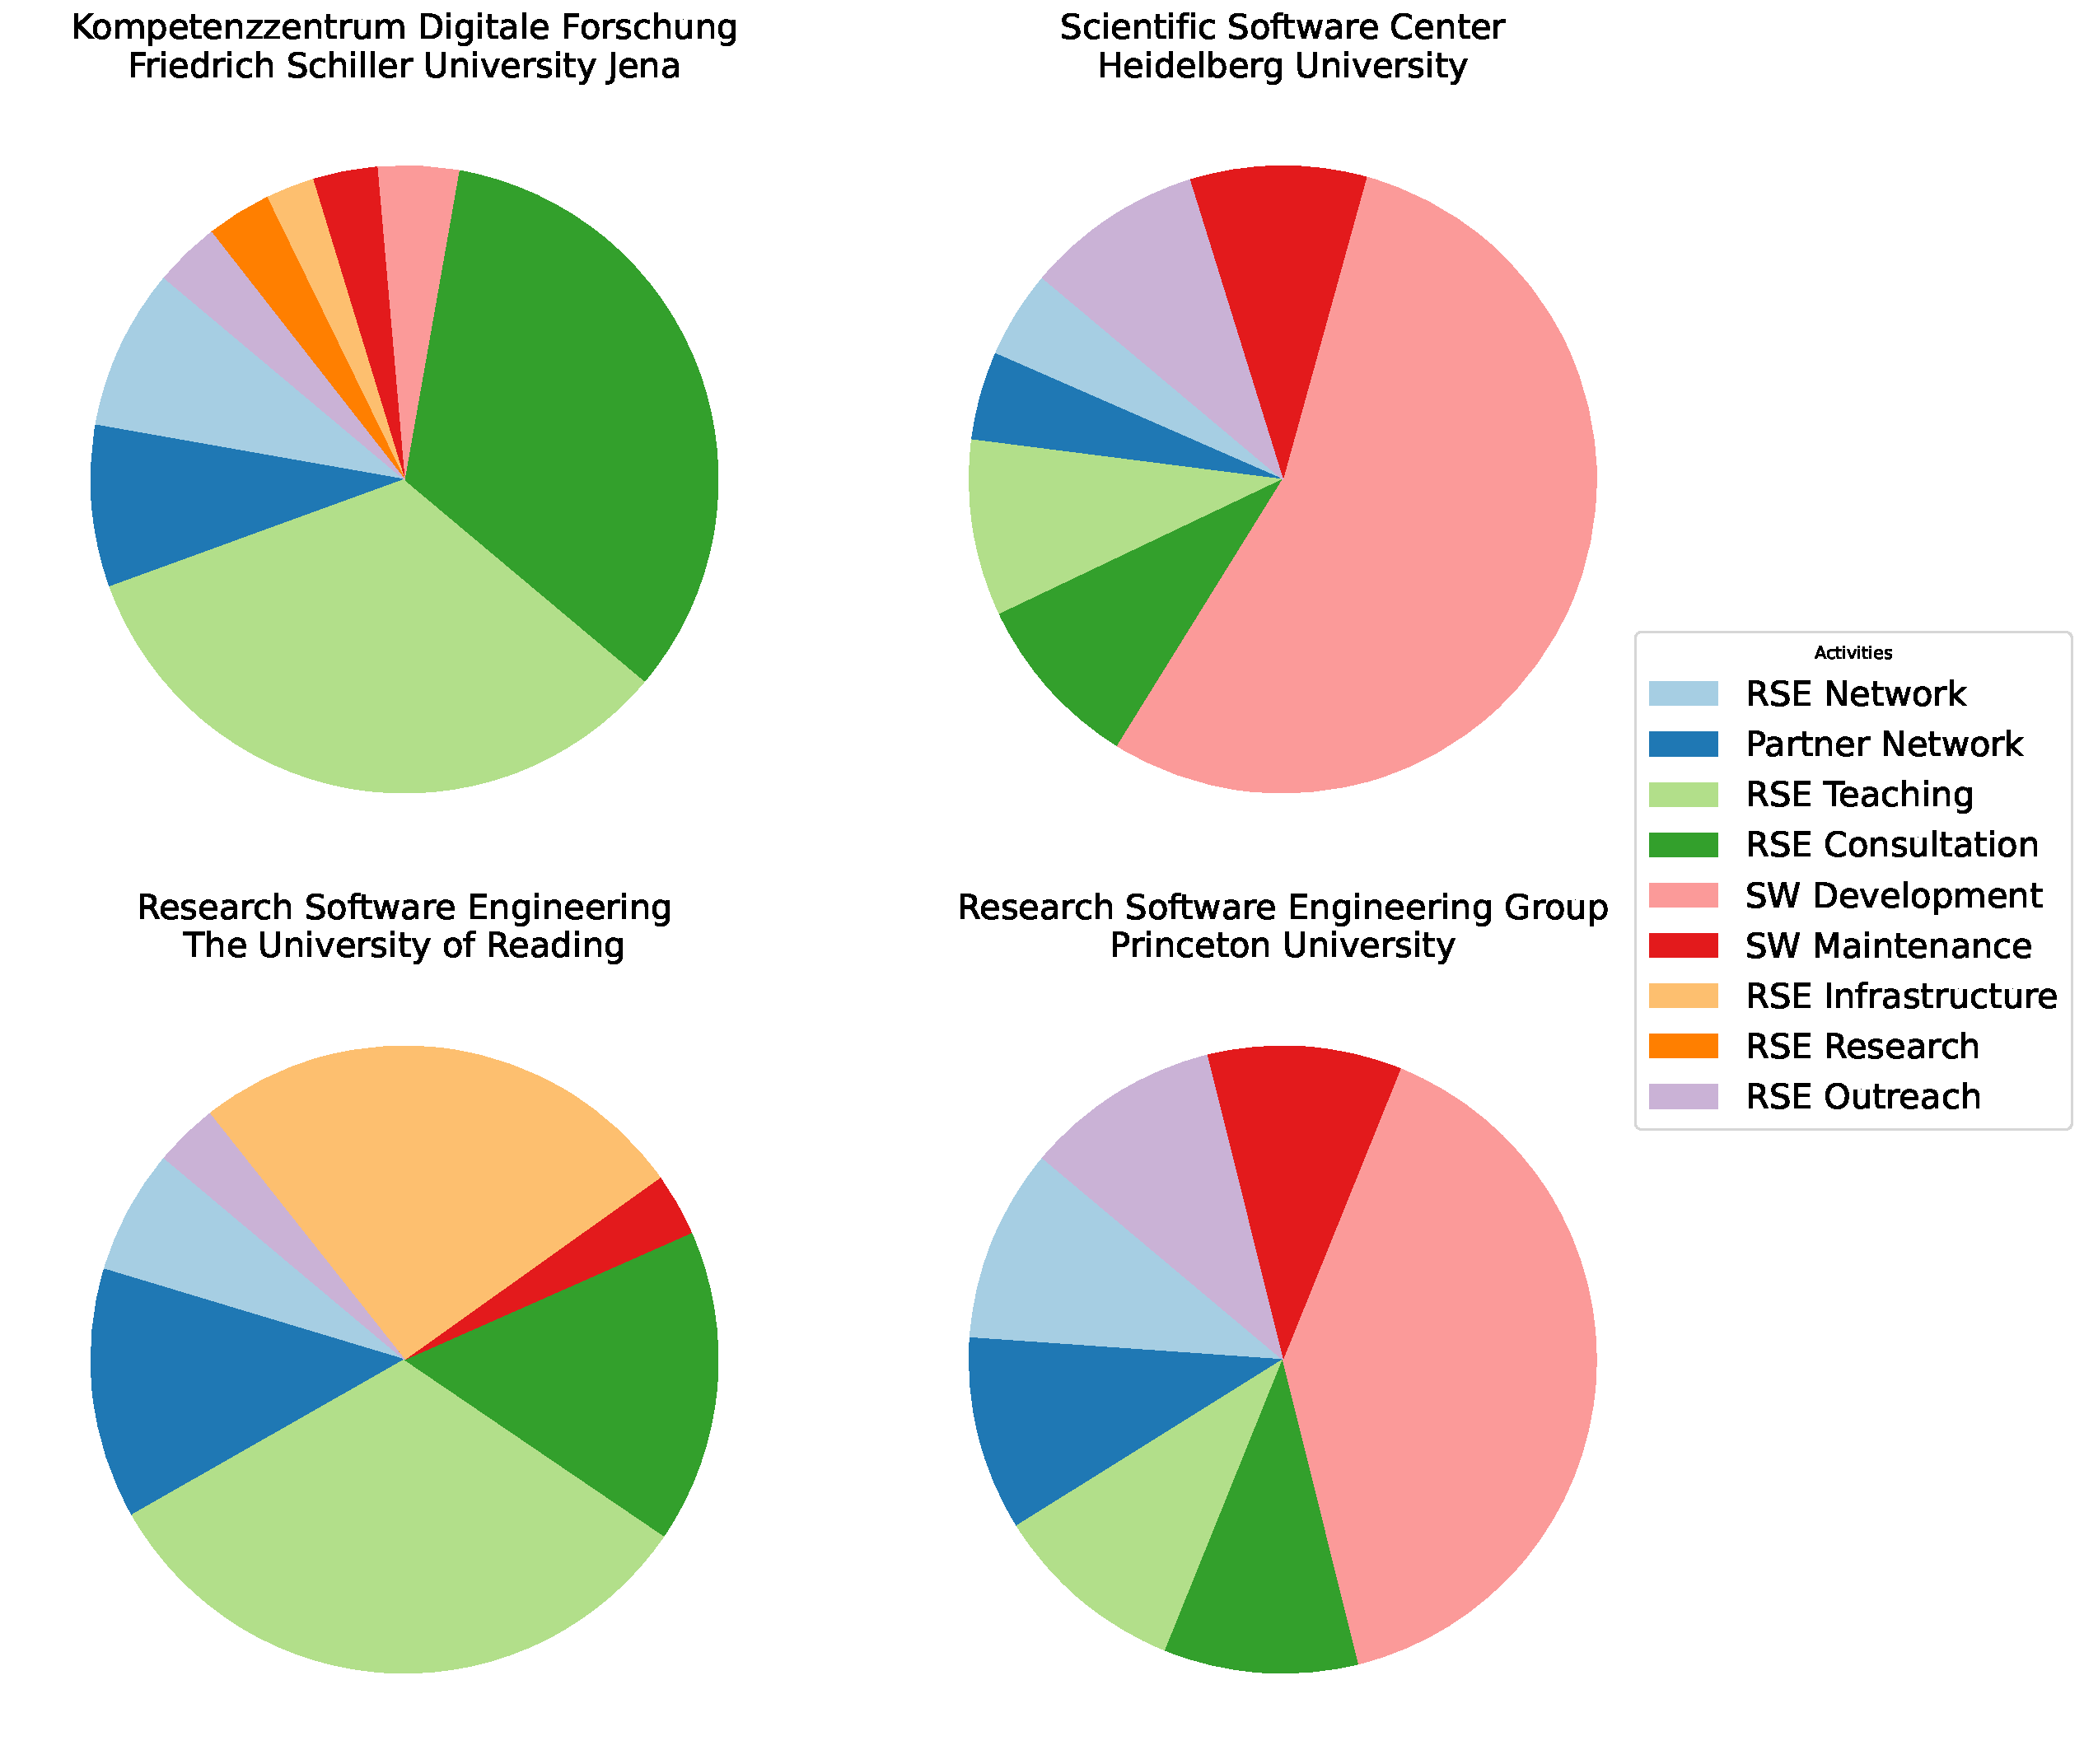
\includegraphics[width=\textwidth]{./group_composition_plot/pdf/group_composition_plot_the_fantastic_four.pdf}
\caption{National and international examples of RSE departments and their service portfolio: Heidelberg and Princeton offer development services, whereas Jena and Reading focus mostly on teaching and consultation services.}
\end{figure}

A number of successful installations of RSE departments already exist in Germany and many more exist in other countries, especially the UK and the US.
In order to understand the service portfolio of these existing RSE departments, we conducted a survey that received a total of twelve responses from Germany, the UK and the US.
We asked departments for the composition of their service portfolio - the results are shown in figure~\ref{fig:survey}.

From the gathered data and the additional free text information of the participants we conclude that the service components that we have identified in section~\ref{sec:vision} are indeed relevant for existing RSE departments.
Additionally, we see a large diversity in the weighting of these components, which is to be expected given the different environments of the RSE departments.
Within this diverse data, we identified two rather different archetypes of RSE departments: Those that offer development services and those that do not.
The departments offering such services would typically invest a lot of their resources into this component, where as others put a much larger emphasis on teaching and consultation services.
We should note however, that our survey did not collect information about the size of the department.
It is likely that the departments offering development services are also larger in size,
and that their total resource commitment to teaching and consultation services is similar to that of the departments that do not offer development services.

When setting up a new RSE department, it is important to find the best service portfolio composition for the local environment.
This depends on the demand by scientists at the institution, existing structures and the available funding.

\section{Realization Strategy}
\label{sec:realization}

We propose a realization strategy for a central institutional RSE department.
We start by listing different possibilities for funding RSE positions at a research institution.
Following that, we describe a potential transition pathway, starting from existing structures that have grown in research alliances such as collaborative research centers or also in research departments of an institution.
This is complemented by discussing the opportunity of outsourcing RSE services and the challenging task of identifying and hiring suitable RSE candidates.

\subsection{Funding Possibilities}
\label{sec:funding}

We see four basic options for financing RSE positions, which we will briefly explain below:
\begin{enumerate}
\item ordinary budget positions,
\item the overhead of externally funded projects,
\item explicitly requested person-months in externally funded projects, and
\item dedicated RSE calls.
\end{enumerate}
While each option stands for itself, in reality, an institutional RSE department will most certainly finance its personnel by an appropriate mixture of possibly all four options.
The mixture at a particular institution depends heavily on the local conditions.

At research institutions, it is important to resolve the conflict between time-limited research funding and the need for permanent positions in order to be competitive with industry.
Experience is also an essential component of software engineering, which makes long-term employment indispensable.
In principle, pooling of positions and funds makes it possible to finance permanent positions from changing and mixed sources.
Nevertheless, convincing the institution to take the corresponding risk of failing to raise external funds may be a very challenging task.
\begin{enumerate}
\item It seems natural to allocate ordinary budget positions for RSEs.
      However, particularly at German universities, it is usually impossible to create completely new budget positions and the only feasible way is to rededicate an existing position after its corresponding holder has left.
      Depending on the local circumstances at an institution, this can be a cumbersome and time-consuming process for each such position.
\item Funding organizations additionally allocate a portion of the direct project funds as overhead, which is typically divided between the institution and the applicant.
      We propose using a small percentage of the overhead agglomorated at the institution to permanently finance central RSE positions.
      Assuming a third-party funding income of EUR 50 million annually and a 20\% overhead, EUR 100,000 in permanent funding requirements for one person-year would only account for 1\% of this overhead.
\item In project applications involving the development of research software, corresponding person-months should be applied for to finance RSE tasks.
      In this way, an applicant can book a fixed number of working hours from the RSE pool and pay for the costs accordingly.
      This model has been successfully implemented at several UK universities.
      In order to scale, it needs to be supported by an institutional policy.
      Large scale collaborative projects can often apply for dedicated technical support positions that align well with the idea of RSE departments.
\item Funding organizations are increasingly recognizing the need for sustainable research software
      development and are setting up correspondingly designated funding programmes.
      The DFG has already organized three calls for proposals in 2016\footnote{\href{https://www.dfg.de/resource/blob/172674/1bcb181a6451fdac9d94421776b52798/161026-dfg-ausschreibung-forschungssoftware-de-data.pdf}{Nachhaltigkeit von Forschungssoftware}}, 2019\footnote{\href{https://www.dfg.de/de/aktuelles/neuigkeiten-themen/info-wissenschaft/2019/info-wissenschaft-19-44}{Qualitätssicherung von Forschungssoftware durch ihre nachhaltige Nutzbarmachung}}, and 2022\footnote{\href{https://www.dfg.de/en/news/news-topics/announcements-proposals/2022/info-wissenschaft-22-85}{Research Software – Quality Assured and Re-usable}}.
      It is to be expected that even more programs will be launched in the future.
      An already established RSE concept at an institution increases the chances of being successful in such calls.
\end{enumerate}

In addition to these funding options, we encourage funding agencies to provide seed funding for the establishment of RSE structures.
Such seed grants ease the local decision making process and give RSEs the leeway to establish collaborations with researchers without the direct need to ask for remuneration.

% We see two possibilities to acquire additional funds.
% Some can come from the convergence of existing central structures.
% Other funds must come from the departments.
% One possibility is that a share of all overheads goes to the RSE department.
% This solution is simple in principle and also immediately makes the department known, but will also require effective reporting to determine the required share.
% However, it might be difficult to realize the required reallocation of resources.
% Another possibility is the pooling of RSE funds from different departments, which brings its own administrative burden, and is probably not generating long-term positions.
% To generate these RSE funds it is required to obtain them from external funders like the DFG, a strategy that can be supported by an institutional policy to ask for these.
% This mixed funding scheme brings us to organizational topics that facilitate the money generation.
% From the side of the funding agencies this can be supported by requiring a digital support strategy from proposals similar to RDM plans.
% If this strategy/policy is followed institution-wide, we believe that a consistent stream of income can be generated that enhances the bare-level support that is generated by the fixed funding from the central budget.

\subsection{Transition Pathway}

We present a possible transition pathway from RSEs distributed over an institution and associated purely with research working groups and corresponding projects towards an institutional RSE department.
After starting with initial measures not necessarily requiring dedicated funding, we discuss the conceptualization phase, followed by the department's foundation, and concluded by measures for promoting its growth.

\subsubsection{Initial Measures}
The following measures initialize the two modules presented in \autoref{sec:network} and \autoref{sec:teaching}.
While dedicated funding certainly is beneficial already for this initialization, it is not mandatory.
Once the two measures are in place, they can be used to illustrate the need for institutional RSE activities and therefore support funding proposals.

\paragraph{Network of RSEs}
Forming a network of RSEs localized at an institution can be initiated by any existing RSE individual or group that is preferably already in contact with other RSEs at the institution.
An institutional dedicated mailing list, chat group and possibly other communication platforms can be created and a request for participation can be circulated via institutional channels such as an employee newsletter.
First common events such as social gatherings or RSE-related seminar talks can be organized and announced via the communication platform.
This process can be accompanied, facilitated and strengthened by founding a local de-RSE chapter.
Such network-building has been successfully initiated and implemented at several German research institutions.

\paragraph{Pooling of existing teaching materials and training offers}
Depending on local RSE efforts, teaching materials and associated training formats are likely to already exist,
distributed over individual institutional groups.
With the established network, the materials can be pooled and joint training can be offered to a wider institutional audience.
This step can be facilitated and formalized by offering introductory courses with a recognized curriculum as provided by the carpentries\footnote{Examples \url{https://software-carpentry.org/lessons/}}
or coderefinery\footnote{Examples \url{https://coderefinery.org/lessons/}}.

\subsubsection{Conceptualization}
Decision makers at an institution usually require a concept upon which they will decide about the installation of an RSE department.
Such a concept should specify the idea of the department, its responsibilities and offerings as a subset of the nine modules presented in \autoref{sec:vision}, and the resulting benefits for the institution and its researchers.

A rather difficult and crucial question can be the localization of the department within the organizational structure of the institution.
A canonical place would be a new subunit of an institutional body close to software,
training services and computing such as the institution's IT department or library.
Since most institutions already have an RDM department, it seems natural to add the RSE department as a parallel structure.
Another choice for the superordinate body, particularly at universities, is the faculty for computer science.
Determining the best place may involve discussing with several stakeholders at the institution and can already be beneficial for creating a
network of institutional partners, the module described in \autoref{sec:partners}.

The concept should also address funding for the department's initial staff.
We consider it necessary that there is a certain amount of base funding provided by the institution that covers a basic RSE department because much RSE work is not project based.
While possibilities can be drawn from the discussion above, specific ideas should be discussed beforehand with the decision makers.
For facilitating the expansion of the department in the longer term, the installment of an institutional policy for requesting person-months in externally funded projects dedicated to RSE should be proposed.

Another part of the concept should be the governance structure of the department.
One of the decisions to be made is if the department head is supposed to be part of the department itself or if the department will be headed by a person outside of it.
Additionally, installing an advisory board can be proposed in the concept, recruiting from the prospective institutional partners.

\subsubsection{Installation of the Department}
Once the concept has been approved by the institution, the RSE department can be installed accordingly.
The initial staffing depends crucially on the local institutional conditions. 
One promising possibility is to start with two positions. The first one would be an RSE coordinator.
They will be the contact person for all institutional RSEs, organizing meetings, developing training programs, reporting to superordinate bodies, etc.
The second position would be a central RSE, responsible for providing selected services and infrastructure.
These central positions will be complemented by the existing RSEs organized in the network to form a pool of institutional RSEs associated with the department.

Drawing from the concept and considering the actual initial staff situation, a first task of the centrally funded structure is to define a basic service portfolio according to the modules described in \autoref{sec:vision}.
In addition to the already mentioned networking and teaching cf.~\autoref{sec:network} and \autoref{sec:teaching}, it seems natural to start with consultation cf.~\autoref{sec:consultation},
as this allows to evaluate the potential necessities for other services such as development, infrastructure provisioning and maintenance.
An extension of the initial service portfolio for a larger target audience requires the acquisition of further funding and installation of further positions, see below.

\subsubsection{Growth of the Department}

\paragraph{Acquisition of further funding}
The most promising possibilities to acquire further funding seem to be explicitly requesting person-months in externally funded projects and dedicated RSE calls, as discussed in \autoref{sec:funding}.
We believe that the credibility of a research proposal that is asking for RSE funds is greatly enhanced if the RSE department is part of this proposal from the beginning.
Over time, more and more researchers and proposals are expected to follow the institutional policy such that a consistent stream of income can be generated.

\paragraph{Offering of additional services}
With the additional acquired funds, the service portfolio of the RSE department can be enhanced regarding the modules described in \autoref{sec:vision}.
Obviously, the selection of modules and their share in the overall portfolio depend on the services that have been applied for in the corresponding proposals.
As this is strongly connected to hiring persons with the required expertise, this has to be carefully planned, see also below.


\subsection{Outsourcing}

Another possibility for the realization of local RSE Service providers is by forming a spin-off and pooling the RSE Skills into an external company, which has benefits but also drawbacks. [\#SuccessStory Outsourcing]
Among the most obvious benefits is that this enables the creation of contracts outside of the WissZeitVG.
This also widens the customer base of the department since the newly founded company may obtain contracts from industry.
If this company is university backed/branded this enables another possibility for a university to interact with the local society. 
But there are drawbacks.
Since the company is now a university external entity the Vergabe-Richtlinien have to be fulfilled, which could e.g. mean to publicly invite tenders in order to have a competitive procedure.
This also points to the fact that an external company has to be a mostly profitable entity (partly this can be softened by founding a non-for-profit entity).
Moreover, during the outsourcing contract, there has to be a coordinator at both sides and the flow of information from the academic institution to the contracted company has to be established.
These are some examples of additional administrative overhead due to the interaction with external partners.
Certain domains will have issues with ensuring data privacy when working with this external company.
If forming a public company, it is hoped that parts of these issues can be legally alleviated by forming respective framework agreements between a university and the company.
It is of particular importance to agree on requirements and handover criteria, including quality assurance and license specifications.
On top of these drawbacks, there are soft factors, like whether an external company is accepted by scientists.

\subsection{Staff Acquisition/People}

This leaves us with the question of, assuming we have centralized RSE departments, where do we get the employees?
Being an RSE should be a career worth aspiring to as any other profession and hence we have to additionally create education structures that generate a pool of people where central RSE departments can be populated from.
This is a topic that will be considered in a separate paper.
These RSEs will bring a diverse set of skills centered around the topics of research, 
digital tools, and team-based work and hence can easily offer the consulting services mentioned in the previous section and guide people to their implementation in their workgroups.
To fill gaps, the RSE department can also maintain a roster of freelance workers.
In order to retain RSEs it should be possible for them to become experts in a field and hence this should make this job more attractive to young RSEs,
in order to mitigate the problem that some will only see this job as a one-year stint after their PhD and then move on to something else.
To facilitate the retention of skilled people, industry has long identified education as an effective tool.
For RSEs this should be helped by to be formed academic facilities that enable them to keep on learning skills after their first professional qualification, supported by the respective certification programs.
In the longer run, Research Software Engineering should be integrated into the existing study programmes.
One option here would be the creation of an RSE master as a specialization for a computer science bachelor.
This should be complemented by adding a minor in application-domain study programs such as biology, physics, engineering etc. to facilitate the communication between the corresponding two groups of RSEs.
There are already some master's programs available, (\eg in Berlin, Munich and Stuttgart) that develop this specialization on top of a domain bachelor.
And of course there are data science curricula in the process of being created. A curated and continuously updated list of these programs is available at \cite{learnandteachlearn}.

%\begin{thebibliography}{9}
%\end{thebibliography}
\printbibliography[heading=bibintoc]

\end{document}
